% !Mode:: "TeX:UTF-8" 

\chapter{示例文档}[Example]

这是 \hithesis\ 的示例文档,基本上覆盖了模板中所有格式的设置。建议大家在使用模板
之前,除了阅读《\hithesis\ 用户手册》,这个示例文档也最好能看一看。
这个示例文档尽量使用到所有的排版格式,然而对于一些不在我工规范中规定的文档,理论
上是由用户自由发挥,这里不给出样例。需要另行载入的宏包和自定义命令在文件
`hithesis.sty'中有示例,这里不列举。

\section{索引示例}[Index]

为便于检索文中内容,可编制索引置于论文之后(根据需要决定是否设置)。索引以论文中
的专业词语为检索线索,指出其相关内容的所在页码。索引用中、英两种文字书写,中文在
前。\sindex[china]{qi!乔峰}\sindex[english]{Xu Zhu}\sindex[english]{Qiao Feng}
中文按各词汉语拼音第一个字母排序,英文按该词第一个英文字母排序。

\subsection{引用}[Cite]

\sindex[china]{du!段誉}引文标注遵照GB/T7714-2005,采用顺序编码制。正文中引用文献的标示应置于所引内容最后一个字的右上角,所引文献编号用阿拉伯数字置于方括号“[ ]”中,用小4号字体的上角标。要求:

(1)引用单篇文献时,如“二次铣削\cite{cnproceed}”。

(2)同一处引用多篇文献时,各篇文献的序号在方括号内全部列出,各序号间用“,”,如
遇连续序号,可标注讫序号。如,…形成了多种数学模型\cite{cnarticle,cnproceed}…

(3)多次引用同一文献时,在文献序号的“[ ]”后标注引文页码。如,…间质细胞CAMP含量
测定\cite[100-197]{cnarticle}…。…含量测定方法规定
\cite[92]{cnarticle}…。

(4)当提及的参考文献为文中直接说明时,则用小4号字与正文排齐,如“由文献\inlinecite{hithesis2017}可知”

\subsection{图片}[Pictures]
图应有自明性。插图应与文字紧密配合,文图相符,内容正确。选图要力求精练,插图、照
片应完整清晰。机械工程图:采用第一角投影法,严格按照GB4457~GB131-83《机械制图》
标准规定。数据流程图、程序流程图、系统流程图等按GB1526-89标准规定。电气图:图形
符号、文字符号等应符合附录3所列有关标准的规定。流程图:必须采用结构化程序并正确
运用流程框图。对无规定符号的图形应采用该行业的常用画法。坐标图的坐标线均用细实线
,粗细不得超过图中曲线;有数字标注的坐标图,必须注明坐标单位。照片图要求主题和主
要显示部分的轮廓鲜明,便于制版。如用放大或缩小的复制品,必须清晰,反差适中。照片
上应有表示目的物尺寸的标度。引用文献中的图时,除在正文文字中标注参考文献序号以外
,还必须在中、英文表题的右上角标注参考文献序号。

\subsubsection{博士毕业论文双语题注}[Doctoral picture example]
\begin{figure}[htpb]
\centering
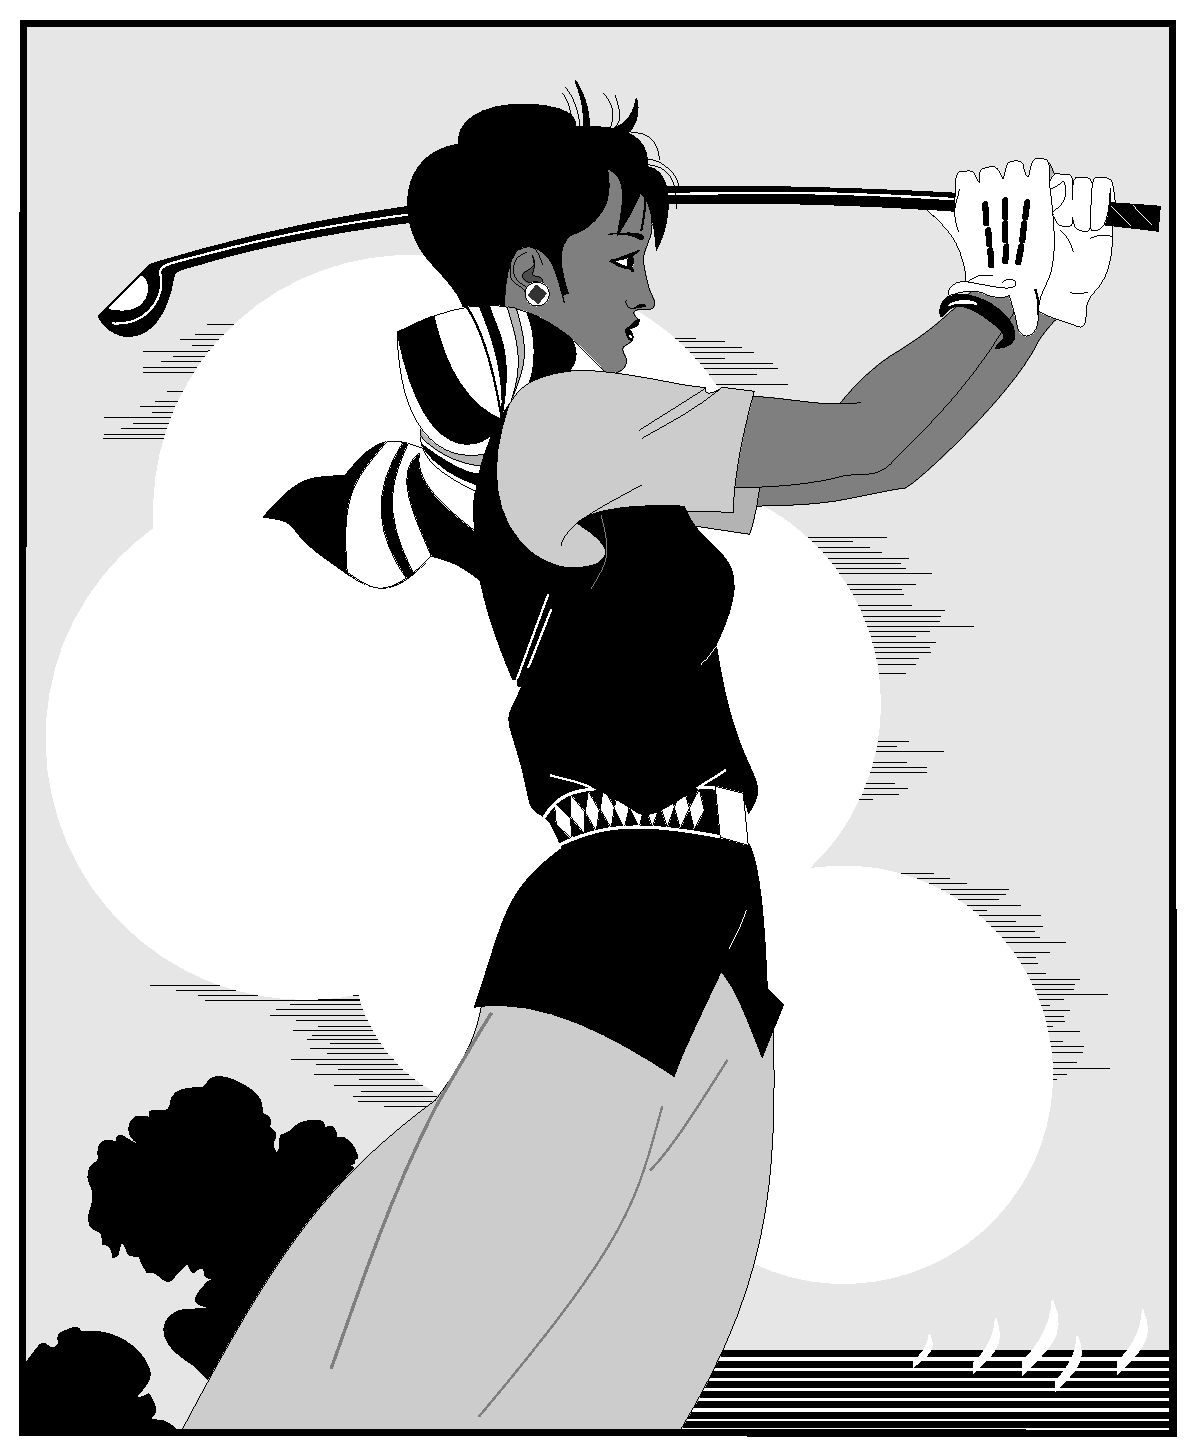
\includegraphics[width = 0.4\textwidth]{golfer}
\bicaption[golfer1]{}{图打打高尔夫球的人打高尔夫球的人打高尔夫球的人打高尔夫球球的人高尔夫球的人球的人高尔夫球的人的人高尔夫球的人}{Fig.$\!$}{The person playing golf playing golf playing golf playing golf playing golf playing golf playing golf playing golf}
\end{figure}

每个图均应有图题(由图序和图名组成),图题不宜有标点符号,图名在图序之后空1个半
角字符排写。图序按章编排,如第1章第一个插图的图号为“图1-1”。图题置于图下,硕士论
文只用中文,博士论文用中、英两种文字,居中书写,中文在上,要求中文用宋体5号字,
英文用Times New Roman 5号字。有图注或其它说明时应置于图题之上。引用图应注明出处
,在图题右上角加引用文献号。图中若有分图时,分图题置于分图之下或图题之下,可以只
用中文书写,分图号用a)、b)等表示。图中各部分说明应采用中文(引用的外文图除外)或
数字符号,各项文字说明置于图题之上(有分图时,置于分图题之上)。图中文字用宋体、
Times New Roman字体,字号尽量采用5号字(当字数较多时可用小5号字,以清晰表达为原
则,但在一个插图内字号要统一)。同一图内使用文字应统一。图表中物理量、符号用斜体
。
\subsubsection{本硕论文题注}[Other picture example]
\begin{figure}[h]
\centering
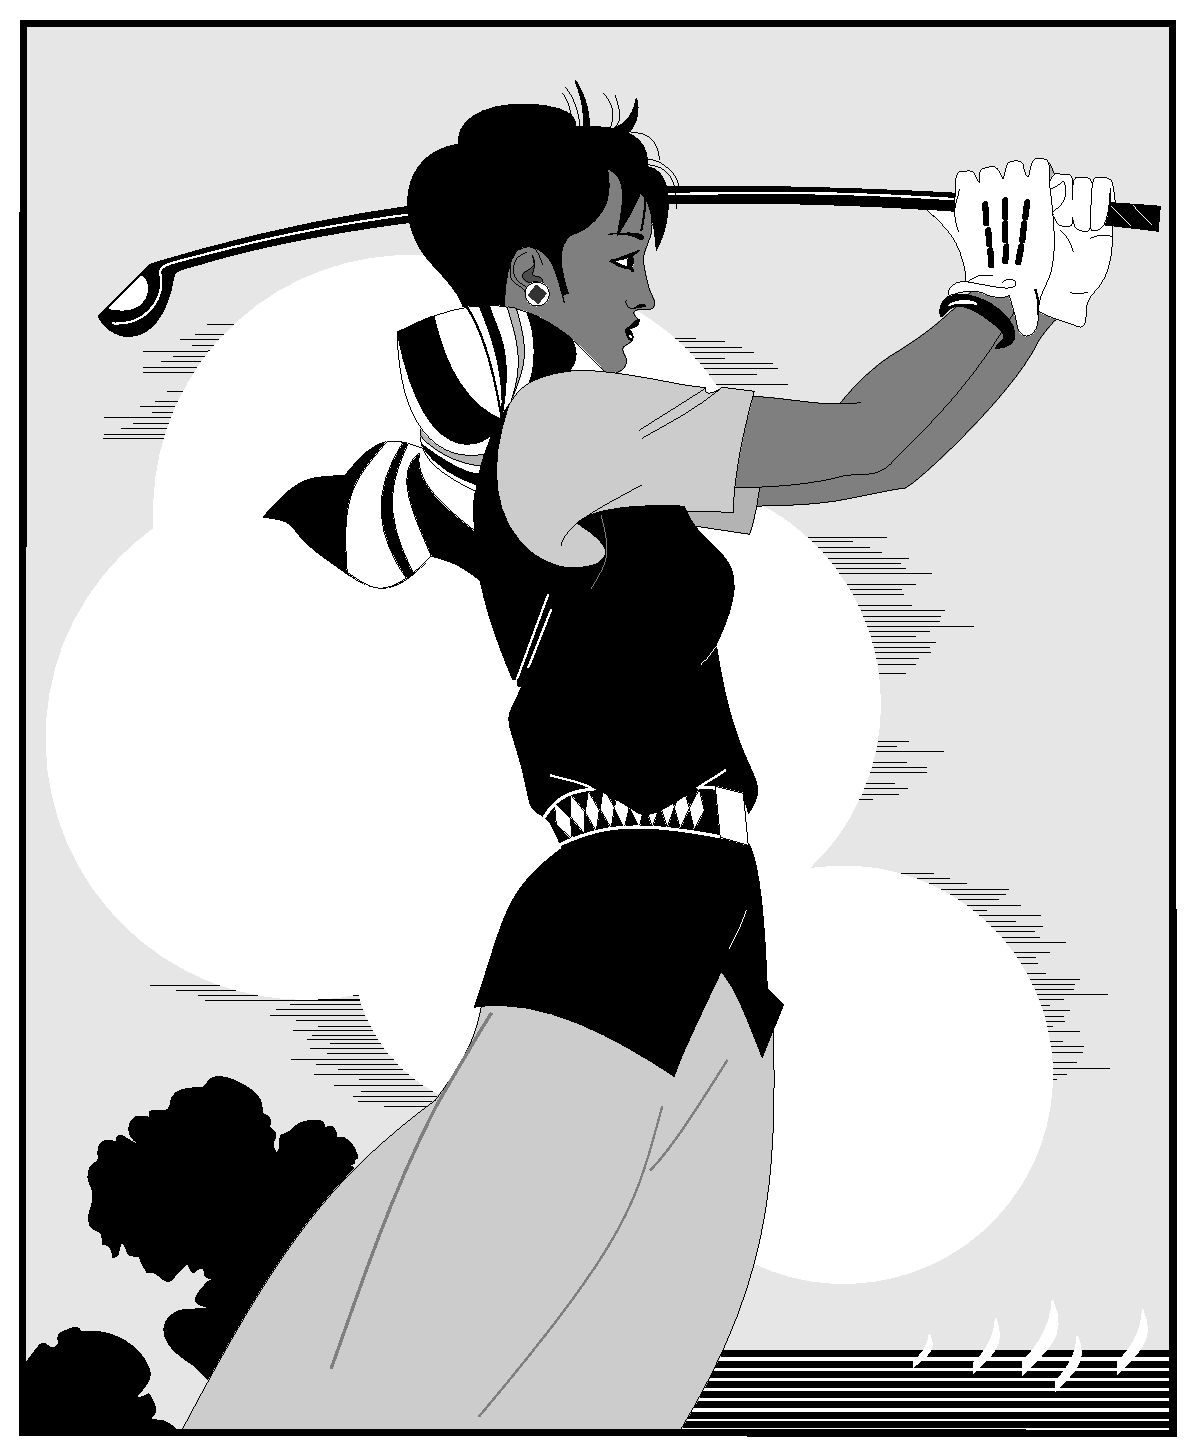
\includegraphics[width = 0.4\textwidth]{golfer}
\caption{打高尔夫球的人}
\end{figure}

\subsubsection{并排图和子图}[Sub-picture example]
注意:子图题注也可以只用中文。

\begin{figure}[htbp]
\centering
\begin{minipage}{0.4\textwidth}
\centering
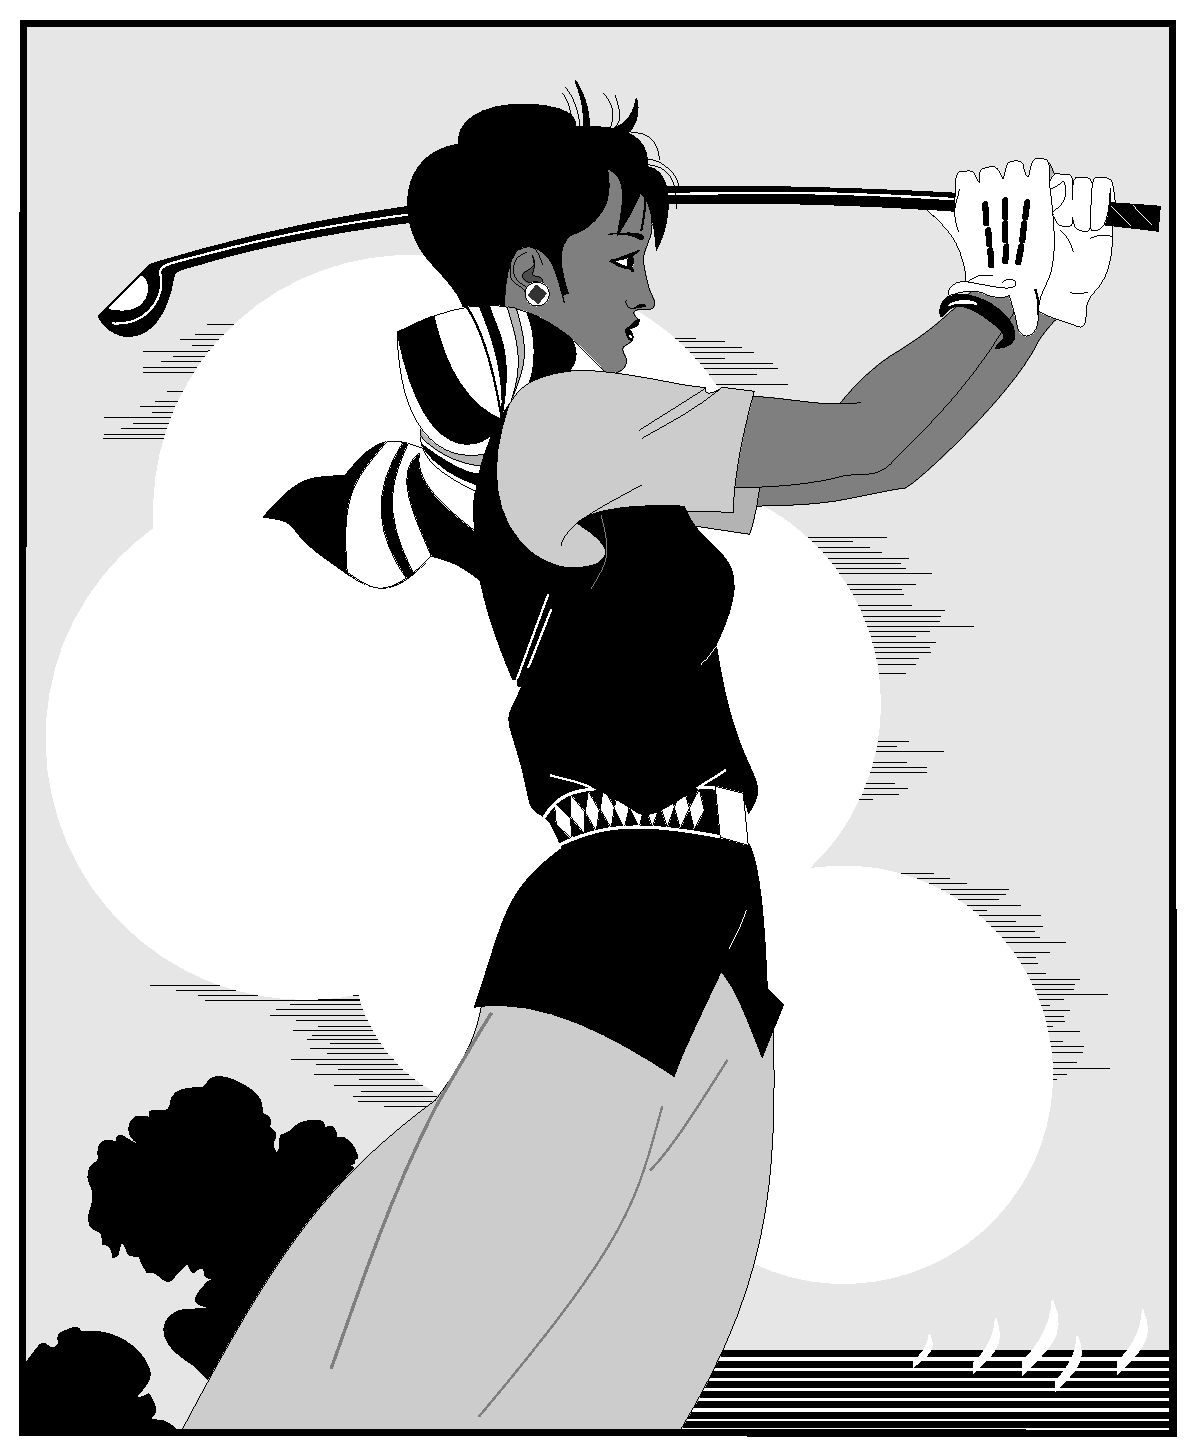
\includegraphics[width=\textwidth]{golfer}
\bicaption[golfer2]{}{打高尔夫球的人}{Fig.$\!$}{The person playing golf}
\end{minipage}
\begin{minipage}{0.4\textwidth}
\centering
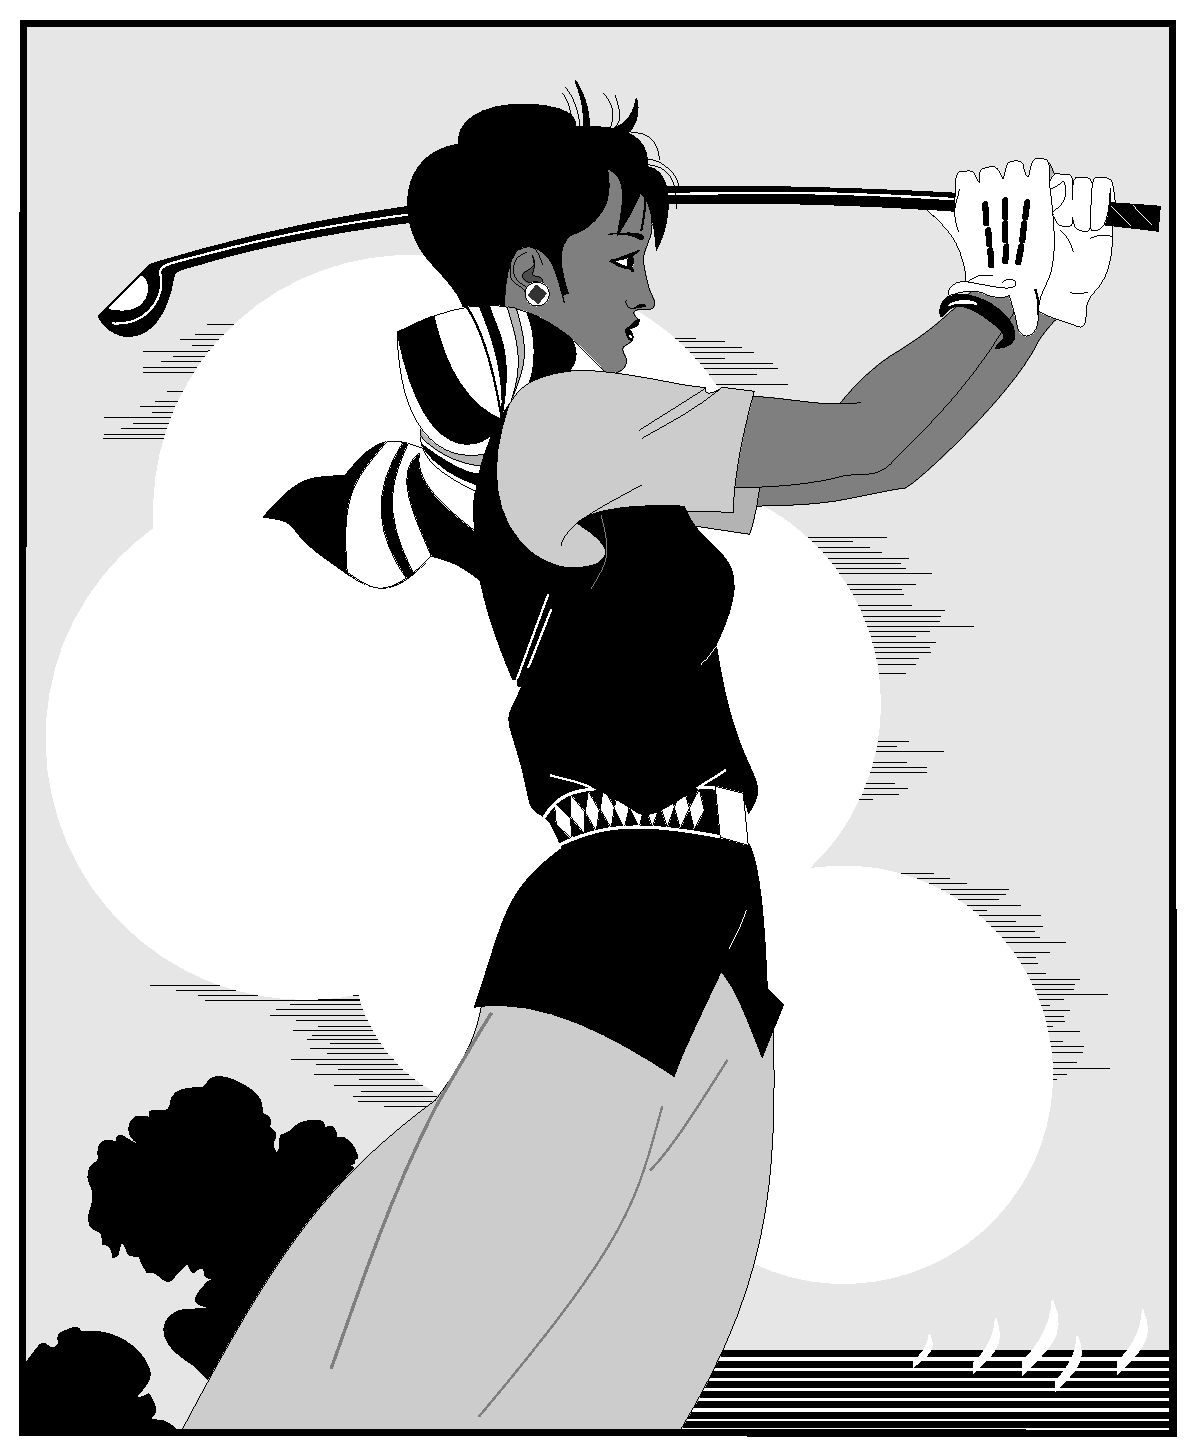
\includegraphics[width=\textwidth]{golfer}
\bicaption[golfer3]{}{打高尔夫球的人}{Fig.$\!$}{The person playing golf}
\end{minipage}
\end{figure}

\begin{figure}[!h]
\setlength{\subfigcapskip}{-1bp}
\centering
\subfigure{\label{golfer41}}\addtocounter{subfigure}{-2}
\subfigure[The person playing golf]{\subfigure[打高尔夫球的人~1]{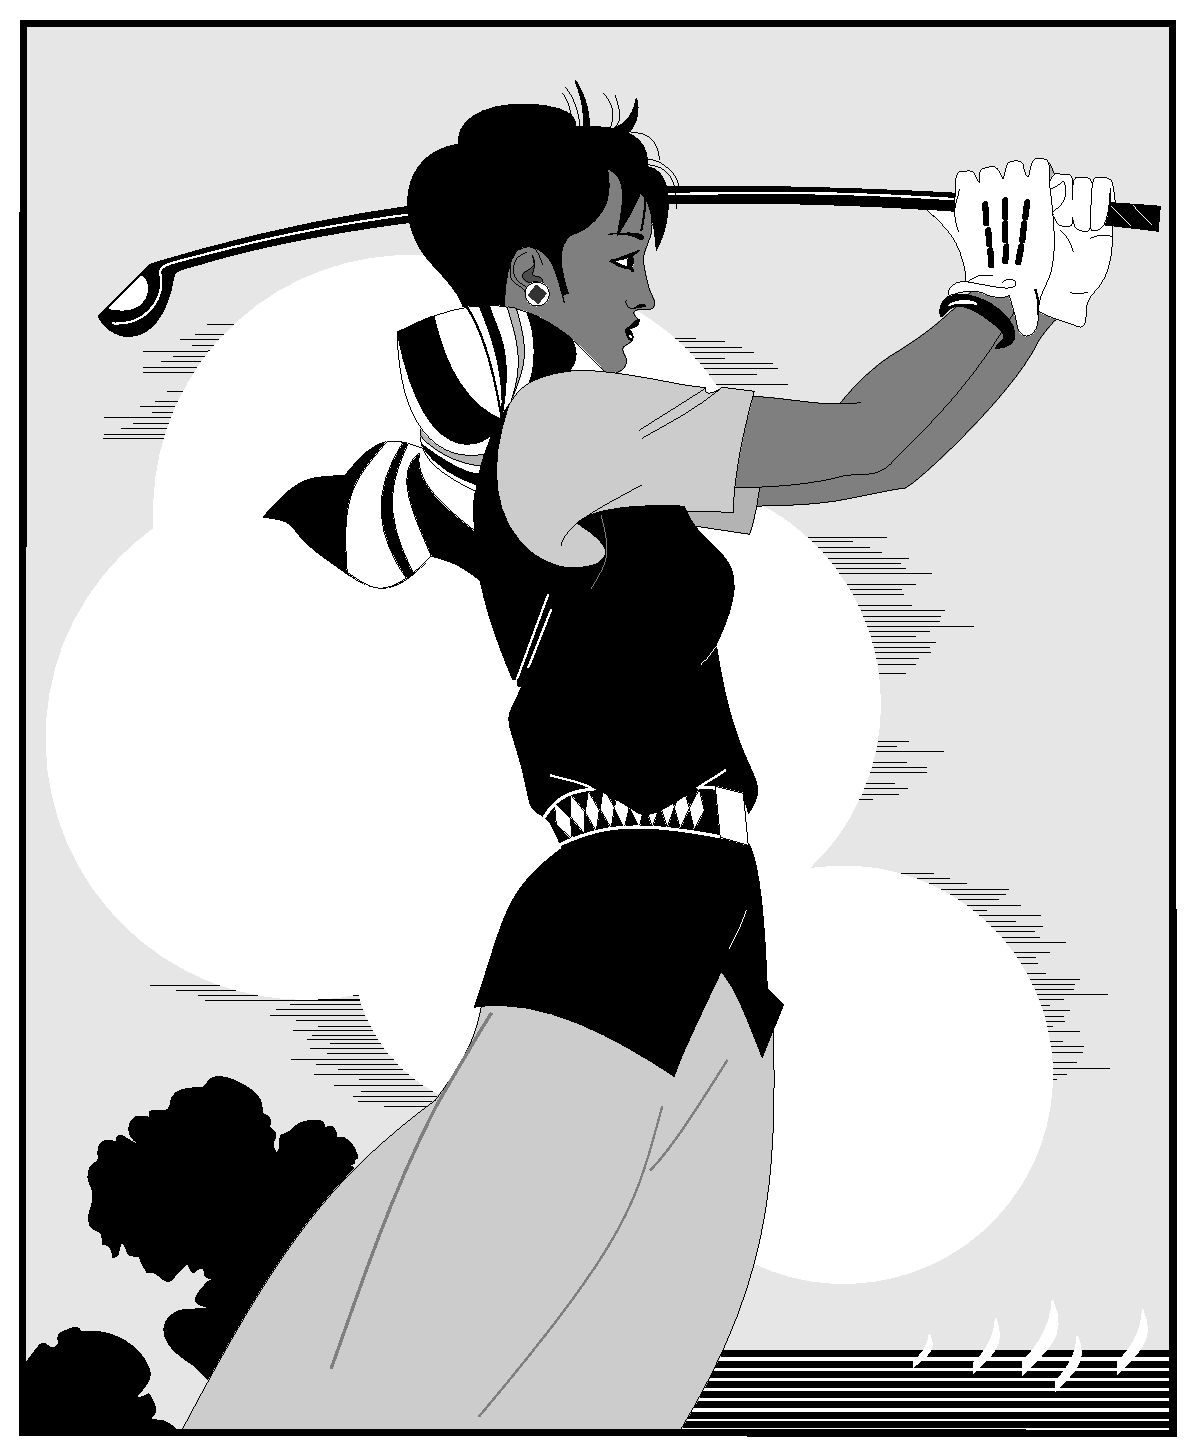
\includegraphics[width=0.4\textwidth]{golfer}}}
\subfigure{\label{golfer42}}\addtocounter{subfigure}{-2}
\subfigure[The person playing golf]{\subfigure[打高尔夫球的人~2]{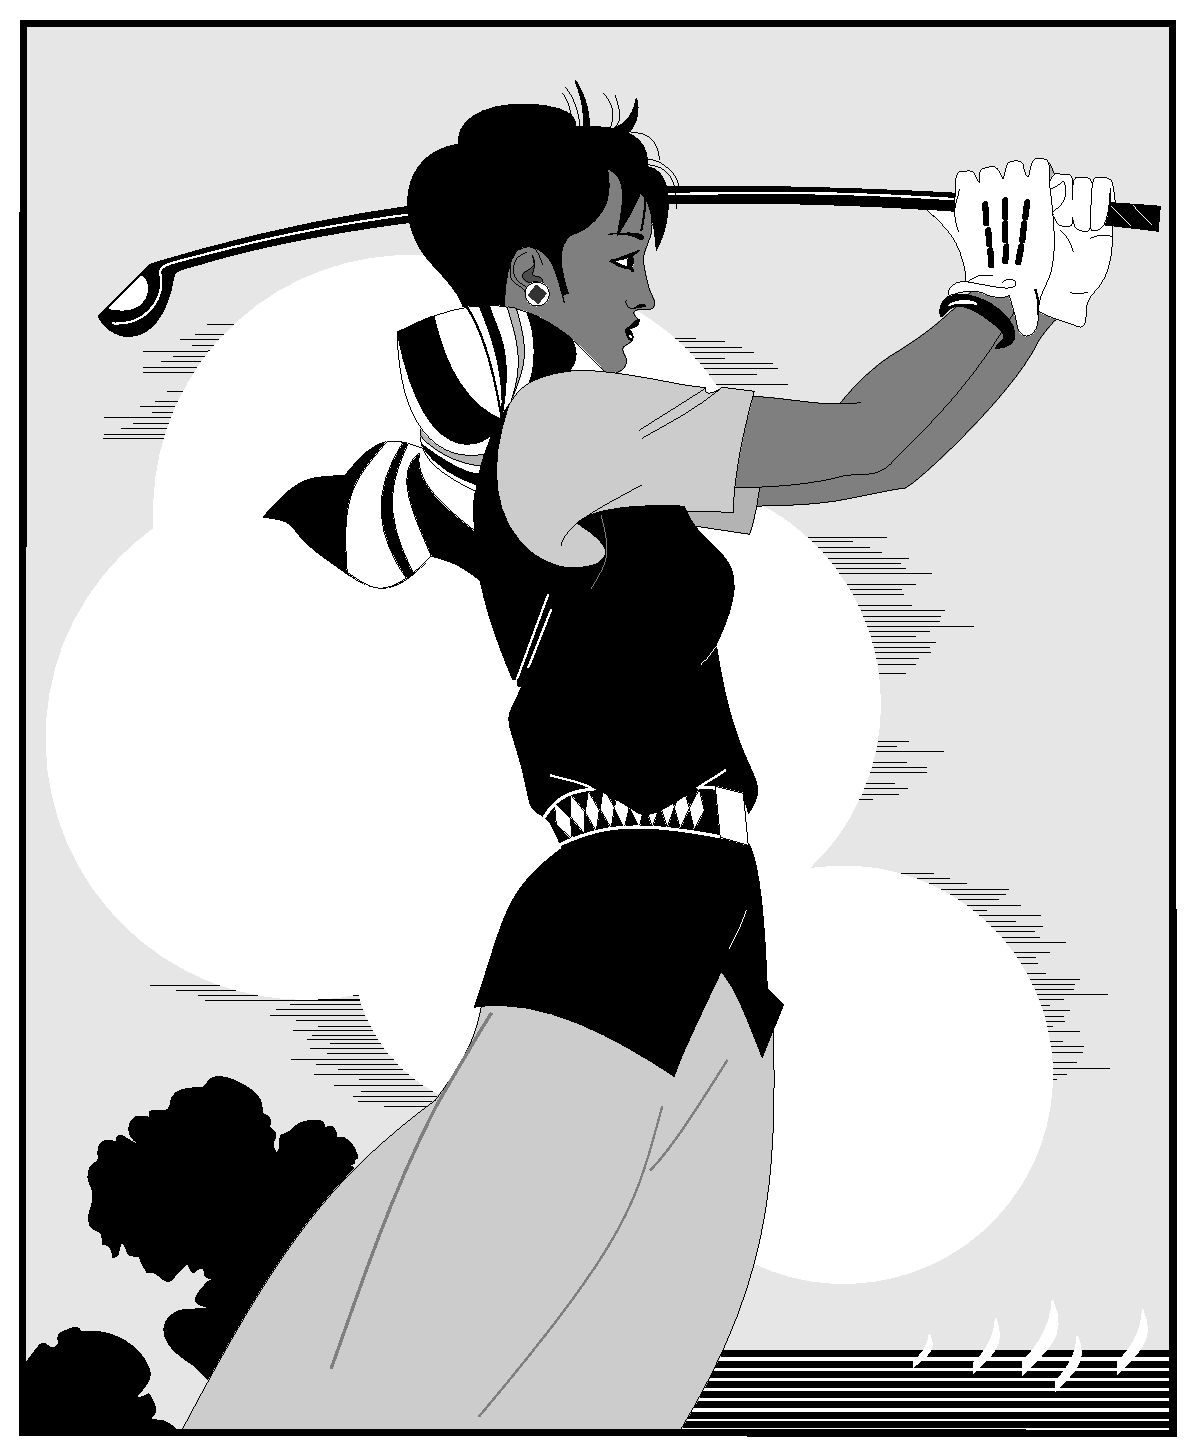
\includegraphics[width=0.4\textwidth]{golfer}}}
\subfigure{\label{golfer43}}\addtocounter{subfigure}{-2}
\subfigure[The person playing golf]{\subfigure[打高尔夫球的人~3]{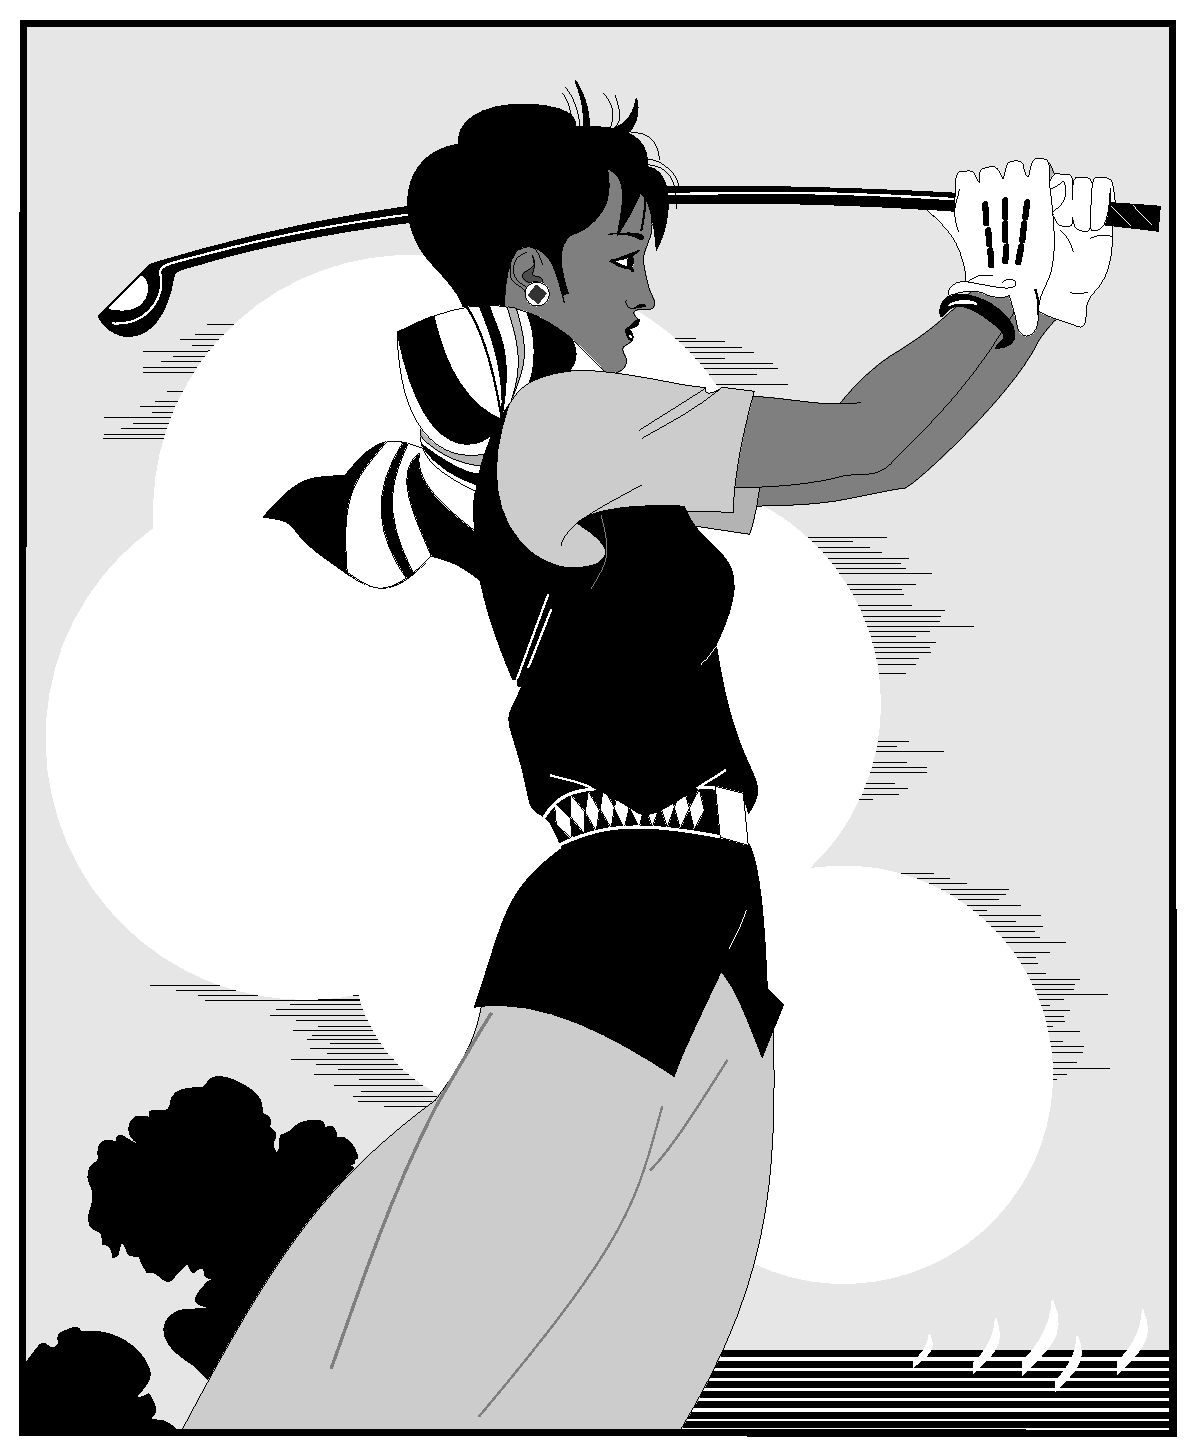
\includegraphics[width=0.4\textwidth]{golfer}}}
\subfigure{\label{golfer44}}\addtocounter{subfigure}{-2}
\subfigure[The person playing golf]{\subfigure[打高尔夫球的人~4]{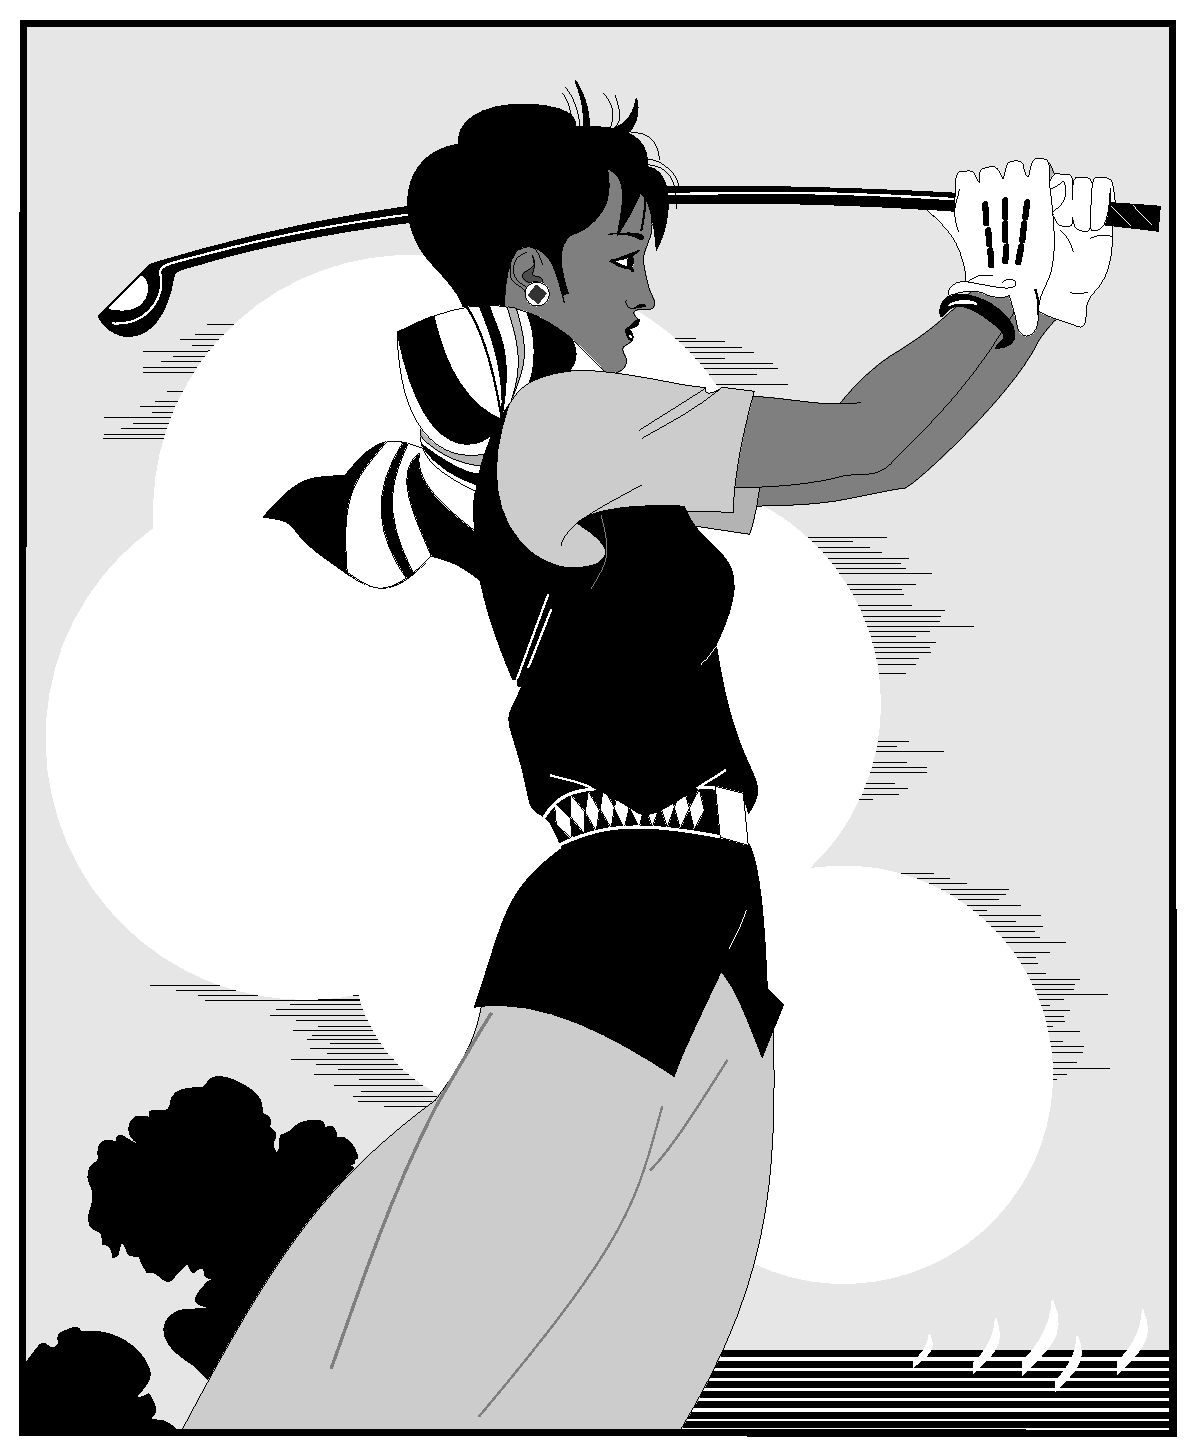
\includegraphics[width=0.4\textwidth]{golfer}}}
\vspace{0.2em}
\bicaption[golfer4]{}{打高尔夫球的人}{Fig.$\!$}{The person playing golf}
\end{figure}


\section{表格}

表应有自明性。表格不加左、右边线。表的编排建议采用国际通行的三线表。表中文字用宋
体~5~号字。每个表格均应有表题(由表序和表名组成)。表序一般按章编排,如第~1~章第
一个插表的序号为“表~1-1”等。表序与表名之间空一格,表名中不允许使用标点符号,表名
后不加标点。表题置于表上,硕士学位论文只用中文,博士学位论文用中、英文两种文字居
中排写,中文在上,要求中文用宋体~5~号字,英文用新罗马字体~5~号字。表头设计应简单
明了,尽量不用斜线。表头中可采用化学符号或物理量符号。


\subsection{普通表格的绘制方法}[Methods of drawing normal tables]

表格应具有三线表格式,因此需要调用~booktabs~宏包,其标准格式如表~\ref{table1}~所示。
\begin{table}[htbp]
\bicaption[table1]{}{符合研究生院绘图规范的表格}{Table$\!$}{Table in agreement of the standard from graduate school}
\vspace{0.5em}\centering\wuhao
\begin{tabular}{ccccc}
\toprule[1.5pt]
$D$(in) & $P_u$(lbs) & $u_u$(in) & $\beta$ & $G_f$(psi.in)\\
\midrule[1pt]
 5 & 269.8 & 0.000674 & 1.79 & 0.04089\\
10 & 421.0 & 0.001035 & 3.59 & 0.04089\\
20 & 640.2 & 0.001565 & 7.18 & 0.04089\\
\bottomrule[1.5pt]
\end{tabular}
\end{table}
全表如用同一单位,则将单位符号移至表头右上角,加圆括号。表中数据应准确无误,书写
清楚。数字空缺的格内加横线“-”(占~2~个数字宽度)。表内文字或数字上、下或左、右
相同时,采用通栏处理方式,不允许用“〃”、“同上”之类的写法。表内文字说明,起行空一
格、转行顶格、句末不加标点。如某个表需要转页接排,在随后的各页上应重复表的编号。
编号后加“(续表)”,表题可省略。续表应重复表头。

\subsection{长表格的绘制方法}[Methods of drawing long tables]

长表格是当表格在当前页排不下而需要转页接排的情况下所采用的一种表格环境。若长表格
仍按照普通表格的绘制方法来获得,其所使用的\verb|table|浮动环境无法实现表格的换页
接排功能,表格下方过长部分会排在表格第1页的页脚以下。为了能够实现长表格的转页接
排功能,需要调用~longtable~宏包,由于长表格是跨页的文本内容,因此只需要单独的
\verb|longtable|环境,所绘制的长表格的格式如表~\ref{table2}~所示。

注意,长表格双语标题的格式。

\ltfontsize{\dawu[1.667]}
\dawu[1.667]\begin{longtable}{ccc}%
\longbionenumcaption{}{{\wuhao 中国省级行政单位一览
}\label{table2}}{Table$\!$}{}{{\wuhao Overview of the provincial administrative
unit of China}}{-0.5em}{3.15bp}\\
%\caption{\wuhao 中国省级行政单位一览}\\
\toprule[1.5pt] 名称 & 简称 & 省会或首府  \\ \midrule[1pt]
\endfirsthead
\multicolumn{3}{r}{表~\thetable(续表)}\vspace{0.5em}\\
\toprule[1.5pt] 名称 & 简称 & 省会或首府  \\ \midrule[1pt]
\endhead
\bottomrule[1.5pt]
\endfoot
北京市 & 京 & 北京\\
天津市 & 津 & 天津\\
河北省 & 冀 & 石家庄市\\
山西省 & 晋 & 太原市\\
内蒙古自治区 & 蒙 & 呼和浩特市\\
辽宁省 & 辽 & 沈阳市\\
吉林省 & 吉 & 长春市\\
黑龙江省 & 黑 & 哈尔滨市\\
上海市 & 沪/申 & 上海\\
江苏省 & 苏 & 南京市\\
浙江省 & 浙 & 杭州市\\
安徽省 & 皖 & 合肥市\\
福建省 & 闽 & 福州市\\
江西省 & 赣 & 南昌市\\
山东省 & 鲁 & 济南市\\
河南省 & 豫 & 郑州市\\
湖北省 & 鄂 & 武汉市\\
湖南省 & 湘 & 长沙市\\
广东省 & 粤 & 广州市\\
广西壮族自治区 & 桂 & 南宁市\\
海南省 & 琼 & 海口市\\
重庆市 & 渝 & 重庆\\
四川省 & 川/蜀 & 成都市\\
贵州省 & 黔/贵 & 贵阳市\\
云南省 & 云/滇 & 昆明市\\
西藏自治区 & 藏 & 拉萨市\\
陕西省 & 陕/秦 & 西安市\\
甘肃省 & 甘/陇 & 兰州市\\
青海省 & 青 & 西宁市\\
宁夏回族自治区 & 宁 & 银川市\\
新疆维吾尔自治区 & 新 & 乌鲁木齐市\\
香港特别行政区 & 港 & 香港\\
澳门特别行政区 & 澳 & 澳门\\
台湾省 & 台 & 台北市\\
\end{longtable}\normalsize

\ltfontsize{\dawu[1.667]}
\dawu[1.667]\begin{longtable}{ccc}%
  \caption{\wuhao 中国省级行政单位一览}\\[0.3em]
\toprule[1.5pt] 名称 & 简称 & 省会或首府  \\ \midrule[1pt]
\endfirsthead
\multicolumn{3}{r}{表~\thetable(续表)}\vspace{0.5em}\\
\toprule[1.5pt] 名称 & 简称 & 省会或首府  \\ \midrule[1pt]
\endhead
\bottomrule[1.5pt]
\endfoot
北京市 & 京 & 北京\\
天津市 & 津 & 天津\\
河北省 & 冀 & 石家庄市\\
山西省 & 晋 & 太原市\\
内蒙古自治区 & 蒙 & 呼和浩特市\\
辽宁省 & 辽 & 沈阳市\\
吉林省 & 吉 & 长春市\\
黑龙江省 & 黑 & 哈尔滨市\\
上海市 & 沪/申 & 上海\\
江苏省 & 苏 & 南京市\\
浙江省 & 浙 & 杭州市\\
安徽省 & 皖 & 合肥市\\
福建省 & 闽 & 福州市\\
江西省 & 赣 & 南昌市\\
山东省 & 鲁 & 济南市\\
河南省 & 豫 & 郑州市\\
湖北省 & 鄂 & 武汉市\\
湖南省 & 湘 & 长沙市\\
广东省 & 粤 & 广州市\\
广西壮族自治区 & 桂 & 南宁市\\
海南省 & 琼 & 海口市\\
重庆市 & 渝 & 重庆\\
四川省 & 川/蜀 & 成都市\\
贵州省 & 黔/贵 & 贵阳市\\
云南省 & 云/滇 & 昆明市\\
西藏自治区 & 藏 & 拉萨市\\
陕西省 & 陕/秦 & 西安市\\
甘肃省 & 甘/陇 & 兰州市\\
青海省 & 青 & 西宁市\\
宁夏回族自治区 & 宁 & 银川市\\
新疆维吾尔自治区 & 新 & 乌鲁木齐市\\
香港特别行政区 & 港 & 香港\\
澳门特别行政区 & 澳 & 澳门\\
台湾省 & 台 & 台北市\\
\end{longtable}\normalsize
此长表格~\ref{table2}~第~2~页的标题“编号(续表)”和表头是通过代码自动添加上去的,无需人工添加,若表格在页面中的竖直位置发生了变化,长表格在第~2~页
及之后各页的标题和表头位置能够始终处于各页的最顶部,也无需人工调整,\LaTeX~系统的这一优点是~word~等软件所无法比拟的。

\subsection{列宽可调表格的绘制方法}[Methods of drawing tables with adjustable-width columns]
论文中能用到列宽可调表格的情况共有两种,一种是当插入的表格某一单元格内容过长以至
于一行放不下的情况,另一种是当对公式中首次出现的物理量符号进行注释的情况,这两种
情况都需要调用~tabularx~宏包。下面将分别对这两种情况下可调表格的绘制方法进行阐述
。
\subsubsection{表格内某单元格内容过长的情况}[The condition when the contents in
some cells of tables are too long]
首先给出这种情况下的一个例子如表~\ref{table3}~所示。
\begin{table}[htbp]
  \centering
\bicaption[table3]{}{最小的三个正整数的英文表示法}{Table$\!$}{The English construction of the smallest three positive integral numbers}\vspace{0.5em}\wuhao
\begin{tabularx}{0.7\textwidth}{llX}
\toprule[1.5pt]
Value & Name & Alternate names, and names for sets of the given size\\\midrule[1pt]
1 & One & ace, single, singleton, unary, unit, unity\\
2 & Two & binary, brace, couple, couplet, distich, deuce, double, doubleton, duad, duality, duet, duo, dyad, pair, snake eyes, span, twain, twosome, yoke\\
3 & Three & deuce-ace, leash, set, tercet, ternary, ternion, terzetto, threesome, tierce, trey, triad, trine, trinity, trio, triplet, troika, hat-trick\\\bottomrule[1.5pt]
\end{tabularx}
\end{table}
tabularx环境共有两个必选参数:第1个参数用来确定表格的总宽度,第2个参数用来确定每
列格式,其中标为X的项表示该列的宽度可调,其宽度值由表格总宽度确定。标为X的列一般
选为单元格内容过长而无法置于一行的列,这样使得该列内容能够根据表格总宽度自动分行
。若列格式中存在不止一个X项,则这些标为X的列的列宽相同,因此,一般不将内容较短的
列设为X。标为X的列均为左对齐,因此其余列一般选为l(左对齐),这样可使得表格美观
,但也可以选为c或r。

\subsubsection{对物理量符号进行注释的情况}[The condition when physical symbols
need to be annotated]

为使得对公式中物理量符号注释的转行与破折号“———”后第一个字对齐,此处最好采用表格
环境。此表格无任何线条,左对齐,且在破折号处对齐,一共有“式中”二字、物理量符号和
注释三列,表格的总宽度可选为文本宽度,因此应该采用\verb|tabularx|环境。由
\verb|tabularx|环境生成的对公式中物理量符号进行注释的公式如式(\ref{eq:1})所示。
\begin{equation}\label{eq:1}
\ddot{\boldsymbol{\rho}}-\frac{\mu}{R_{t}^{3}}\left(3\mathbf{R_{t}}\frac{\mathbf{R_{t}\rho}}{R_{t}^{2}}-\boldsymbol{\rho}\right)=\mathbf{a}
\end{equation}
\begin{tabularx}{\textwidth}{@{}l@{\quad}r@{———}X@{}}
式中& $\boldsymbol{\rho}$ &追踪飞行器与目标飞行器之间的相对位置矢量;\\
&  $\boldsymbol{\ddot{\rho}}$&追踪飞行器与目标飞行器之间的相对加速度;\\
&  $\mathbf{a}$   &推力所产生的加速度;\\
&  $\mathbf{R_t}$ & 目标飞行器在惯性坐标系中的位置矢量;\\
&  $\omega_{t}$ & 目标飞行器的轨道角速度;\\
&  $\mathbf{g}$ & 重力加速度,$=\frac{\mu}{R_{t}^{3}}\left(
3\mathbf{R_{t}}\frac{\mathbf{R_{t}\rho}}{R_{t}^{2}}-\boldsymbol{\rho}\right)=\omega_{t}^{2}\frac{R_{t}}{p}\left(
3\mathbf{R_{t}}\frac{\mathbf{R_{t}\rho}}{R_{t}^{2}}-\boldsymbol{\rho}\right)$,这里~$p$~是目标飞行器的轨道半通径。
\end{tabularx}\vspace{3.15bp}
由此方法生成的注释内容应紧邻待注释公式并置于其下方,因此不能将代码放入
\verb|table|浮动环境中。但此方法不能实现自动转页接排,可能会在当前页剩余空间不够
时,全部移动到下一页而导致当前页出现很大空白。因此在需要转页处理时,还请您手动将
需要转页的代码放入一个新的\verb|tabularx|环境中,将原来的一个\verb|tabularx|环境
拆分为两个\verb|tabularx|环境。

\section{公式}
与正常\LaTeX\ 使用方法一致,此处略。关于公式中符号样式的定义在`hithesis.sty'有示
例。

\section{其他杂项}[Miscellaneous]

\subsection{算法}[Algorithms]
我工算法有以下几大特点。

(1)算法不再规范中要求。

(2)算法常常被使用(至少计算机学院)。

(3)格式乱,甚至出现了每个实验室的格式要求都不一样。

此处不给出示例,因为没法给,在
\href{https://github.com/dustincys/PlutoThesis}{https://github.com/dustincys/PlutoThesis}
的readme文件中有不同实验室算法要求说明。

\subsection{脚注}[Footnotes]
不再规范\footnote{规范是指\PGR\ 和\UGR}中要求,模板默认使用清华大学的格式。

\subsection{源码}[Source code]
也不再规范中要求。如果有需要最好使用minted包,但在编译的时候需要添加“
-shell-escape”选项且安装pygmentize软件,这些不在模板中默认载入,如果需要自行载入
。

\subsection{专业绘图工具}[Processional drawing tool]
推荐使用tikz包,使用tikz源码绘图的好处是,图片中的字体与正文中的字体一致。具体如
何使用tikz绘图不属于模板范畴。

tikz适合用来画不需要大量实验数据支撑示意图。但R语言等专业绘图工具具有画出各种、
专业、复杂的数据图。R语言中有tikz包,能自动生成tikz码,这样tikz几乎无所不能。

\subsection{术语词汇管理}[Manage glossaries]
推荐使用glossaries包管理术语、缩略语,可以自动生成首次全写,非首次缩写。

\subsection{\TeX\ 源码编辑器}[\TeX editor]
推荐:(1)付费软件Winedt;(2)免费软件kile;(3)vim或emaces或sublime等神级编
译器(需要配置)。

\subsection{\LaTeX\ 排版重要原则}[\LaTeX\ typesetting rules]
格式和内容分离是\LaTeX\ 最大优势,所有多次出现的内容、样式等等都可以定义为简单命
令、环境。这样的好处是方便修改、管理。例如,如果想要把所有的表示向量的符号由粗体
\cs{mathbf}变换到花体\cs{mathcal},只需修改该格式的命令的定义部分,不需要像MS
word那样处处修改。总而言之,使用自定义命令和环境才是正确的使用\LaTeX\ 的方式。
